In this section, we overview the existing approaches to Knowledge Base Question Answering (KBQA), as our approach, described in the next section, builds upon and extends some of these efforts. 

Recently, KBQA systems have converged to two major approaches: {\em semantic parsing}, and {\em information extraction} (IE) \cite{yao2014freebase}.
The former focuses on question understanding, and attempts to parse the sentences into a semantic representation, \eg logical forms \cite{Berant:EMNLP13,berant2014semantic,berant2015imitation}. IE approaches \cite{ACCU:2015,yih2015semantic,yao2014information} are based on identifying \textit{topical entities} in the question, and then, using pre-defined templates for mapping the question to predicates, explore the neighborhood of these entities in a KB.
Theoretically, semantic parsing-based systems would be capable of generating any required queries, and would apply to any question, seen or unseen in training, whereas the template-based approach is less likely to generalize. In practice, however, answers to most of the questions lie within two edge traversals in a KB, making the template (``information extraction''-based) approaches quite effective.

Interestingly, one of the reasons for recent resurgence of interest in KBQA can be credited to creation of the WebQuestions dataset \cite{Berant:EMNLP13}, which is large enough to allow both comprehensive evaluation, and training machine learning methods.
Thus, the performance of KBQA systems has quickly improved, with the current state of the art systems using the IE approach, with sophisticated ranking and matching postprocessing \cite{yih2015semantic}.
In this work, we chose to extend an existing informtion extraction KBQA system -- Aqqu \cite{ACCU:2015} -- which achieves one of the highest scores among publicly available systems.
However, as we will show, our approach is general and can be incorporated into other IE-based systems as well.

%One of the most popular benchmark datasets for knowledge base question answering is WebQuestions \cite{Berant:EMNLP13}, which has attracted a lot of attention recently and as a result the performance increased from 0.357 \cite{Berant:EMNLP13} to 0.525 \cite{yih2015semantic} in average F1 over test questions.
%The dataset is based on Freebase, which has been recently shut down\footnote{https://goo.gl/SZC3tg}.
%The shutdown of Freebase means that it will no longer be extended, but all the data will be available and it will be merged with WikiData\footnote{https://www.wikidata.org/}.
%Therefore, future datasets should probably use different reference KB, but there is no problem in using Freebase for experiments on existing benchmarks, such as WebQuestions.
%We should also stress, that the proposed approach isn't tied to Freebase and can be applied for question answering over dbPedia, WikiData or other knowledge bases.

%The focus of this work is on the fusion between structured data in the KB and unstructured text data.
%Therefore, we chose to extend an existing KBQA system: Aqqu \cite{ACCU:2015}.
%It follows an information extraction approach to KBQA and achieves one of the highest scores among publicly available systems.
%However, our approach can be incorporated into other systems as well.

We will first describe an information extraction approach to KBQA in more detail using Aqqu -- our baseline system -- as an example.
In Section \ref{section:method} we present our system Text2KB, which extends this approach by incorporating external text-based data on various stages of the question answering process.

\begin{figure*}[!ht]
\centering
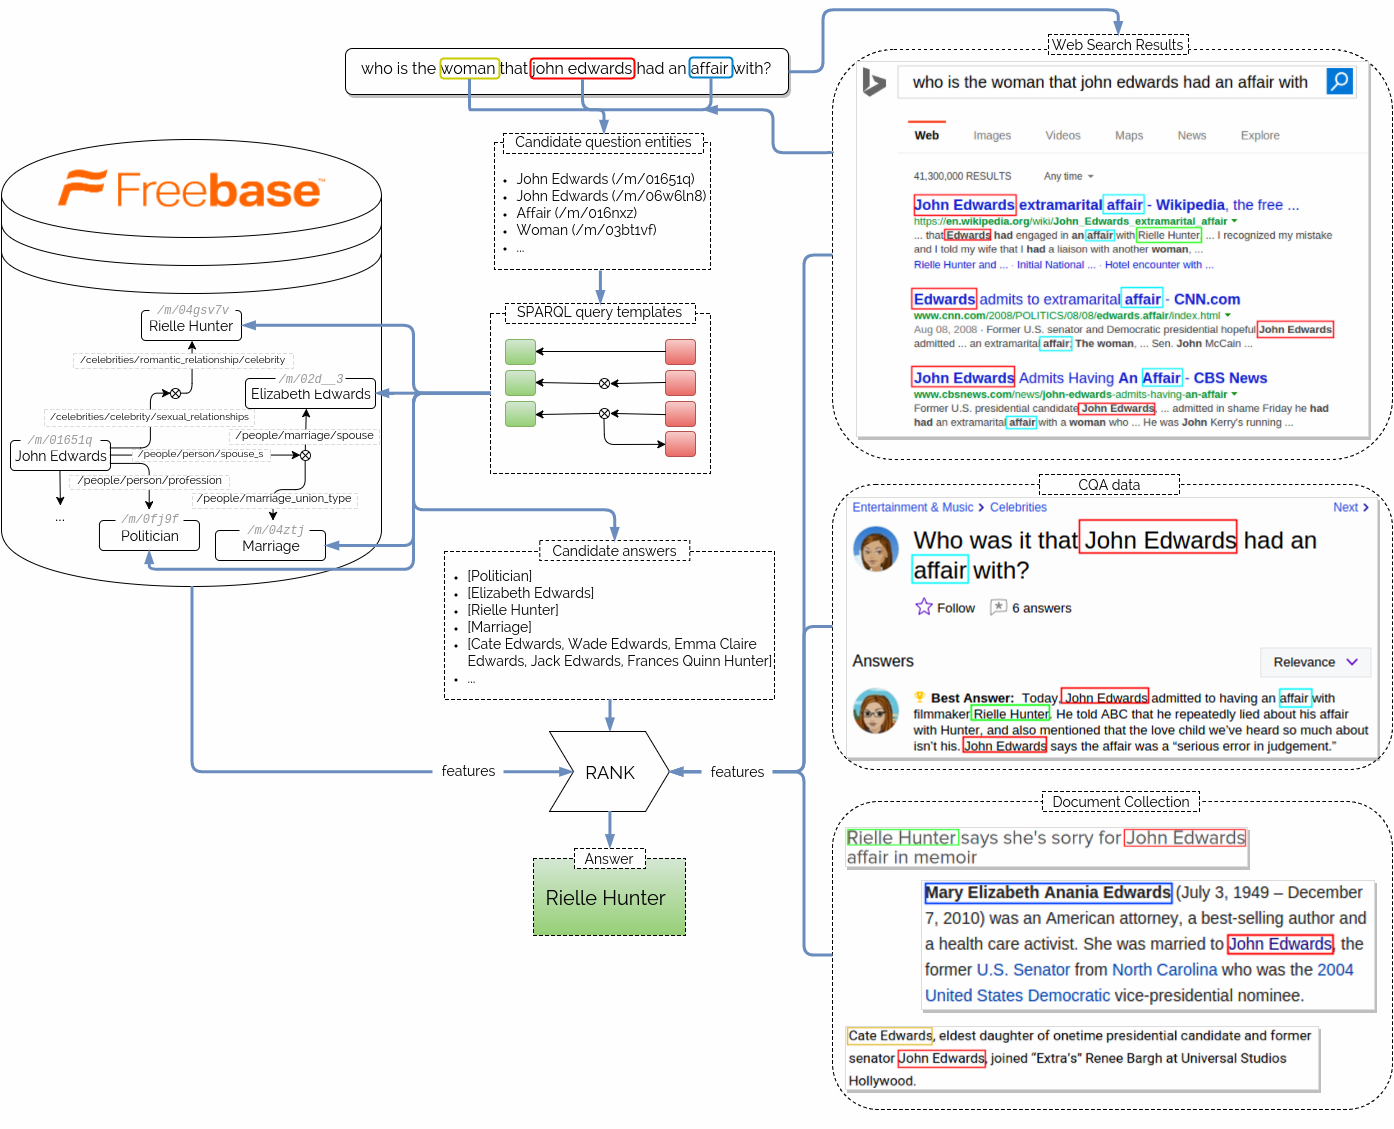
\includegraphics[width=0.9\textwidth]{img/Text2KB_model}
\caption{The architecture of our Text2KB Question Answering system}
\label{fig:model}
\end{figure*}


\subsection{The Aqqu KBQA system}
\label{sec:baseline:aqqu}

First, a KBQA system needs to identify question entities, which are used as sources for the answer search process.
For concreteness, consider a question from the WebQuestions dataset \textit{``who is the woman that john edwards had an affair with?''}.
In this example, entity \texttt{John Edwards} with Freebase mid \texttt{/m/01651q} is the main question entity.
However, Freebase contains millions of entities and it's often hard to identify the topical ones (\eg entities \texttt{Woman} and \texttt{Affair} are also present in Freebase), or to disambiguate and choose between \texttt{John Edwards} a politician (\texttt{/m/01641q}), \texttt{John Edwards} an American racing driver (\texttt{/m/06zs089}) and other people with the same name.
% There is even an entity with the name ``\texttt{had an affair with}''\footnote{http://www.freebase.com/m/0c0n01x}.
Aqqu considers all spans of question words under certain conditions on part of speech tags and uses a dictionary of names, aliases and anchor texts \cite{SPITKOVSKY12.266} to map phrases to potential entities.
Most recent systems, including Aqqu, don't disambiguate entities at this stage and keep a set of candidates along with some information about their popularities (number of triples in the KB, or number of mentions in the collection) and mention scores $p(entity| mention\ text)$.

On the next stage, SPARQL query candidates are generated by exploring the neighborhood of the question topical entities using a predefined set of query templates.
Each query template has question entities, predicate and answer placeholders.
Majority of the answers in WebQuestions dataset can be covered by just 3 templates (q\_entity - question entity, a\_entity - answer entity, cvt\_node - Freebase mediator node, which represent tuples with more than 2 arguments):

\begin{lstlisting}[frame=single,basicstyle=\small]
SELECT DISTINCT ?a_entity {
   <q_entity> <predicate> ?a_entity .
}
\end{lstlisting}

\vspace{-0.25cm}
\begin{lstlisting}[frame=single,basicstyle=\small]
SELECT DISTINCT ?a_entity {
   <q_entity> <predicate_1> ?cvt_node .
   ?cvt_node <predicate_2> ?a_entity .
}
\end{lstlisting}

\vspace{-0.25cm}
\begin{lstlisting}[frame=single,basicstyle=\small]
SELECT DISTINCT ?a_entity {
   <q_entity_1> <predicate_1> ?cvt_node .
   ?cvt_node <predicate_2> <q_entity_2> .
   ?cvt_node <predicate_3> ?a_entity .
}
\end{lstlisting}

The first template retrieves a set of entities that are directly connected to the given question entity via a certain predicate.
The second template accounts for the presence of a mediator node, that groups together arguments of a multi-argument relation.
And the last template looks for cases, when a question also mentions another argument of a multi-argument relation, \eg \texttt{Captain Kirk} and \texttt{Star Trek} for the question \textit{``who played captain kirk in star trek movie?''}.

Each query candidate is represented with a set of features, that includes the scores for linked question entities, various scores for matching between question term n-grams and query predicates, the size of the results list, \etc \cite{ACCU:2015}.
The final stage of the question answering process is filtering and ranking, using a random forest model, built on the training part of the WebQuestions dataset.

\subsection{Basic system extensions}
\label{sec:baseline:extensions}
Before introducing our text-based improvements, described in Section~\ref{section:method}, we introduced some basic improvements to the original Aqqu system.
First, we noticed that since Aqqu does not use information about answer entity Freebase types, in many cases it returns an answer that is incompatible with the question: \eg state instead of county \etc
Therefore, we a trained a model to return a score, measuring a compatibility between the question and answer entities, based on the entity notable types and question uni- and bigrams as features, similar to Aqqu's relations score model.
A second extension introduced a new date range query template, which helps to solve the cases like \textit{``what team did david beckham play for in 2011?''}, where we need to look at the ranges of dates to figure out in which range does the specified date falls.

\begin{lstlisting}[frame=single,basicstyle=\small]
SELECT DISTINCT ?a_entity {
   <q_entity_1> <predicate_1> ?cvt_node .
   ?cvt_node <from_predicate> ?date_from .
   ?cvt_node <to_predicate> ?date_to .
   ?cvt_node <predicate_2> ?a_entity .
   FILTER ( <question_date> >= ?date_from AND
            <question_date> <= ?date_to )
}
\end{lstlisting}

%We also experimented with an additional template, which filters out lists by the entity notable types.

